\documentclass[border=2mm]{standalone}
\usepackage{tikz}
\usepackage{pgfplots}
\pgfplotsset{compat=1.18}

\begin{document}

% Código TikZ mejorado basado en técnicas de R-bloggers
% Referencia: "Some LaTeX Gems – Part 1: TikZ, Loops and more"
% Técnica: Usar coordenadas calculadas para funciones discontinuas

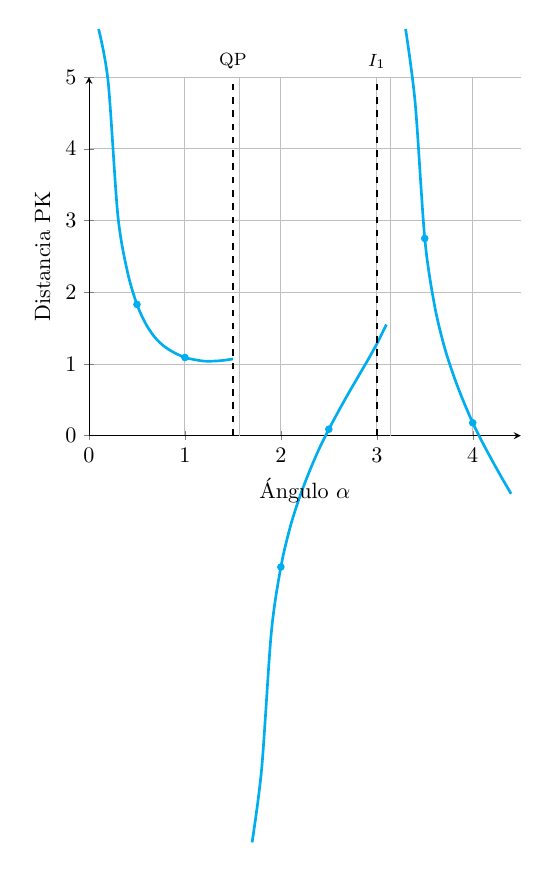
\begin{tikzpicture}[scale=0.8]
\begin{axis}[
    xlabel={Ángulo $\alpha$},
    ylabel={Distancia PK},
    xmin=0, xmax=4.5,
    ymin=0, ymax=5,
    grid=major,
    axis lines=left,
    clip=false
]

% TÉCNICA DE R-BLOGGERS: Usar coordenadas pre-calculadas para evitar problemas
% con funciones discontinuas como cotangente

% Primera rama de la cotangente (0.1 a 1.5, antes de π/2)
\addplot[cyan, very thick, smooth] coordinates {
    (0.1,5.67) (0.2,4.93) (0.3,3.08) (0.4,2.29) (0.5,1.83) 
    (0.6,1.54) (0.7,1.35) (0.8,1.23) (0.9,1.15) (1.0,1.09) 
    (1.1,1.06) (1.2,1.04) (1.3,1.04) (1.4,1.05) (1.5,1.07)
};

% Segunda rama de la cotangente (1.7 a 3.1, entre π/2 y π)
\addplot[cyan, very thick, smooth] coordinates {
    (1.7,-5.67) (1.8,-4.64) (1.9,-2.75) (2.0,-1.83) (2.1,-1.26) 
    (2.2,-0.84) (2.3,-0.49) (2.4,-0.18) (2.5,0.09) (2.6,0.34) 
    (2.7,0.58) (2.8,0.81) (2.9,1.04) (3.0,1.28) (3.1,1.55)
};

% Tercera rama de la cotangente (3.3 a 4.4, después de π)
\addplot[cyan, very thick, smooth] coordinates {
    (3.3,5.67) (3.4,4.64) (3.5,2.75) (3.6,1.83) (3.7,1.26) 
    (3.8,0.84) (3.9,0.49) (4.0,0.18) (4.1,-0.09) (4.2,-0.34) 
    (4.3,-0.58) (4.4,-0.81)
};

% Líneas punteadas verticales (elementos clave de la imagen original)
\draw[dashed, black, thick] (axis cs:1.5,0) -- (axis cs:1.5,5) 
    node[above, black] {\footnotesize QP};
\draw[dashed, black, thick] (axis cs:3.0,0) -- (axis cs:3.0,5) 
    node[above, black] {\footnotesize $I_1$};

% Asíntotas verticales en las discontinuidades
% π/2 ≈ 1.5708, π ≈ 3.1416
\draw[gray!50, very thin] (axis cs:1.5708,0) -- (axis cs:1.5708,5);
\draw[gray!50, very thin] (axis cs:3.1416,0) -- (axis cs:3.1416,5);

% Puntos importantes marcados en la curva
\addplot[cyan, mark=*, mark size=1.5pt, only marks] coordinates {
    (0.5,1.83) (1.0,1.09) (2.0,-1.83) (2.5,0.09) (3.5,2.75) (4.0,0.18)
};

\end{axis}
\end{tikzpicture}

\end{document}
